\documentclass[12pt,a4paper]{report}
\setlength\textwidth{145mm}
\setlength\textheight{247mm}
\setlength\oddsidemargin{15mm}
\setlength\evensidemargin{15mm}
\setlength\topmargin{0mm}
\setlength\headsep{0mm}
\setlength\headheight{0mm}
\setlength{\parindent}{4em}

\let\openright=\clearpage


\usepackage[czech]{babel}

\usepackage[utf8]{inputenc}

\usepackage{indentfirst}
\usepackage{graphicx}
\usepackage{color}
\usepackage{pdfpages}

\usepackage{amsthm}
\usepackage{setspace}

\usepackage[unicode]{hyperref}  
\hypersetup{pdftitle=Název práce}
\hypersetup{pdfauthor=Jméno Příjmení}


\makeatletter
\def\@makechapterhead#1{
  {\parindent \z@ \raggedright \normalfont
   \Huge\bfseries \thechapter. #1
   \par\nobreak
   \vskip 20\p@
}}
\def\@makeschapterhead#1{
  {\parindent \z@ \raggedright \normalfont
   \Huge\bfseries #1
   \par\nobreak
   \vskip 20\p@
}}
\makeatother


\def\chapwithtoc#1{
\chapter*{#1}
\addcontentsline{toc}{chapter}{#1}
}

\begin{document}


\lefthyphenmin=2
\righthyphenmin=2


\pagestyle{empty}
\begin{center}

\large

{ \bf ČESKÁ ZEMĚDĚLSKÁ UNIVERZITA V PRAZE}

\medskip

FAKULTA ŽIVOTNÍHO PROSTŘEDÍ

\medskip

{\sc \Large katedra vodního hospodářství a~environmentálního modelování}

\vfill

\vfill

{\LARGE Vizualizace enviromentálních dat}

\vspace{2mm}

{\bf \Large BAKALÁŘSKÁ PRÁCE}

\vspace{15mm}

\vfill

\vfill

\begin{tabular}{rl}

\noalign{\vspace{2mm}}
Vedoucí práce: & \bf doc. Ing. Martin Hanel, Ph.D. \\
\noalign{\vspace{2mm}}
Bakalant: & \bf Irina Georgievová \\
\end{tabular}

\vfill

2018

\end{center}
\newpage
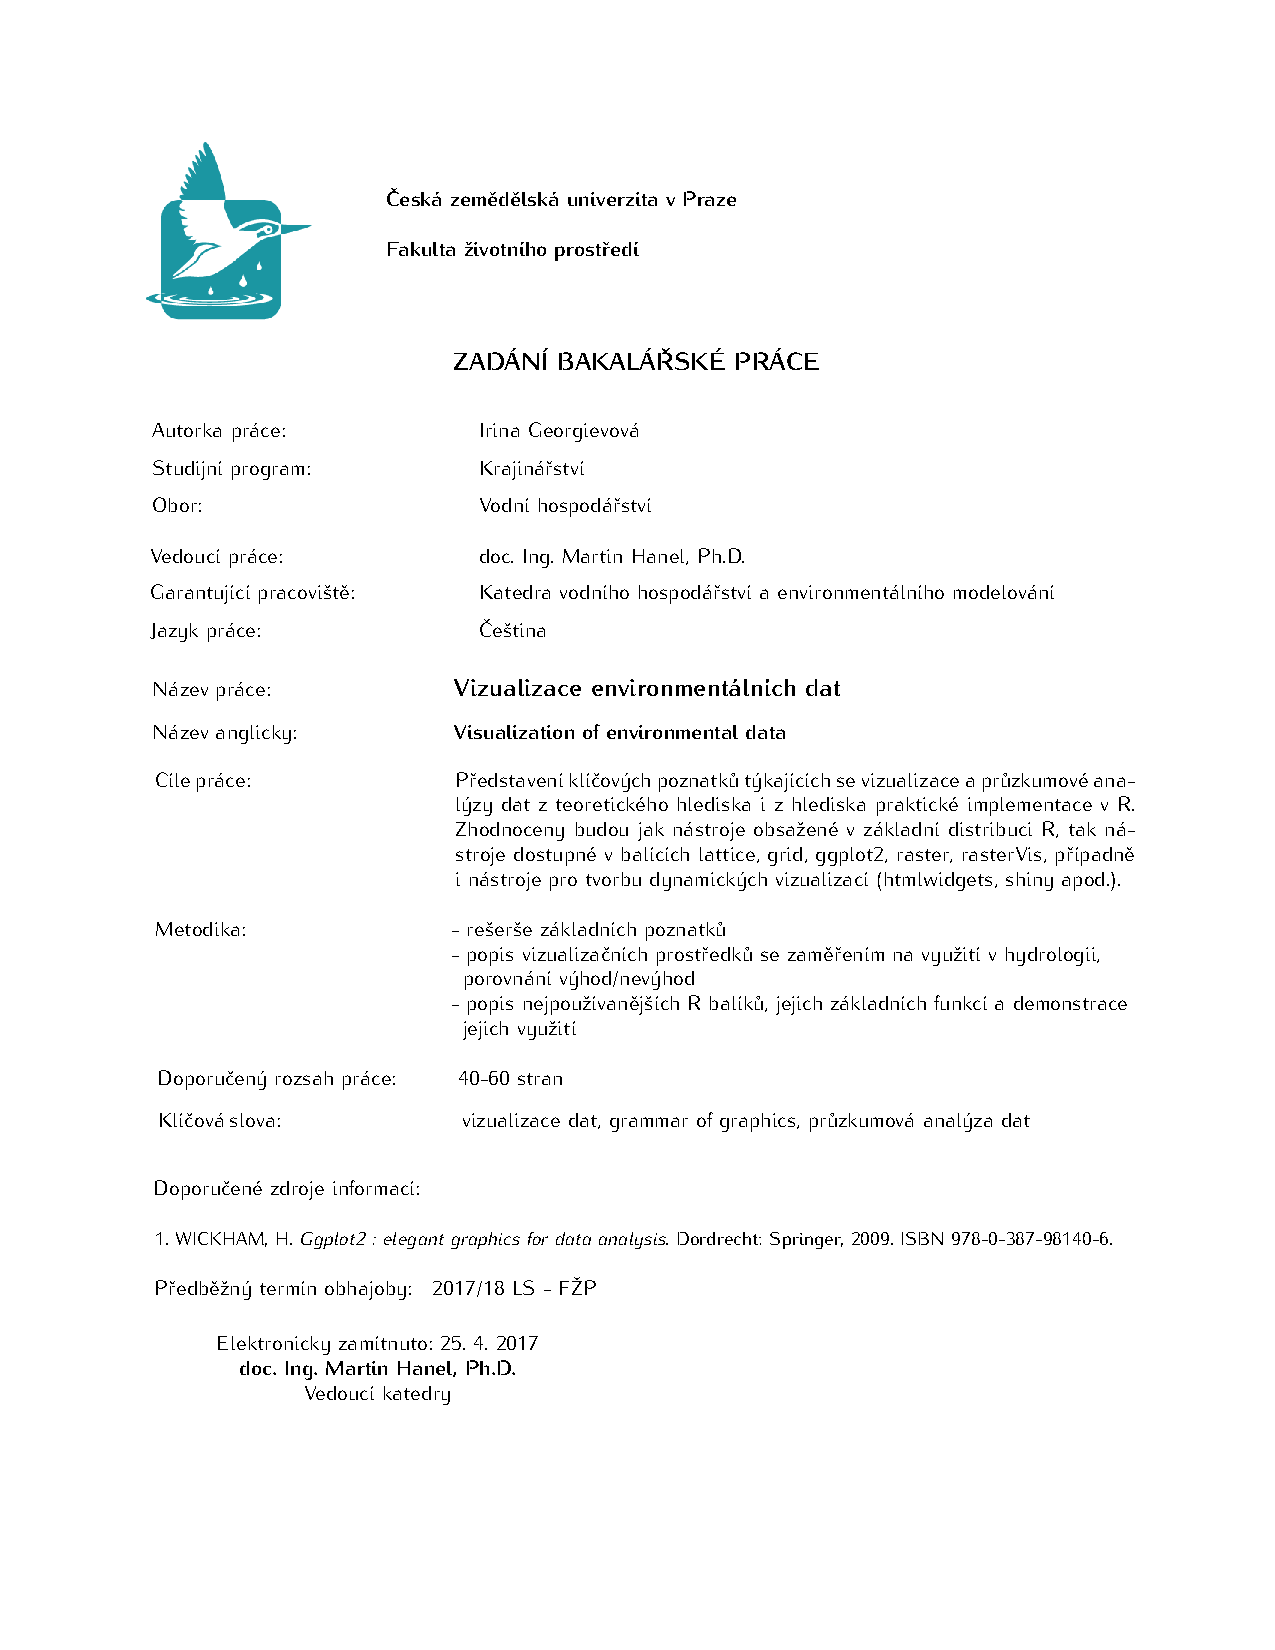
\includepdf[pages={1,2},pagecommand={}, scale = 0.75]{zadani.pdf}
\newpage


\vglue 0pt plus 1fill

\noindent
{\bfseries Prohlášení:} \\
Prohlašuji, že jsem bakalářskou práci \emph{Vizualizace enviromentálních dat} zpracovala samostatně. Veškerou literaturu a další podkladové materiály uvádím v~ seznamu na straně ~\pageref{literatura}.

\vspace{10mm}

\hbox{\hbox to 0.5\hsize{%
V Praze dne ..................
\hss}\hbox to 0.5\hsize{%
\hspace{100pt}...........................
\hss}}

\vspace{1mm}
\hbox{\hbox to 0.5\hsize{%

\hss}\hbox to 0.5\hsize{%
\hspace{100pt}Irina Georgievová
\hss}}

\vspace{20mm}

\newpage

\vglue 0pt plus 1fill
\noindent
{\bfseries Poděkování:} \\

\newpage

\newpage


\vbox to 0.5\vsize{
\setlength\parindent{0mm}
\setlength\parskip{5mm}

{\LARGE\bfseries Abstrakt} 

Práce shrnuje důležité poznatky o vizualizaci dat. Probírá historii jejího vývoje vizualizace a položení vědeckých základů Williamem S. Clevelandem, Edwardem Tuftem a Lelandem Wilkinsonem.  Vizualizace dat je klíčovým nástrojem pro průzkumovou analýzu dat, který je využíván pro jejich lepší pochopení, odhalení neočekávaného chování dat či při rozhodnutí o dalším směru analýzy. Práce dále popisuje nástroje současné  vizualizace dat v programovacím jazyku R a probírá jak základní možnosti softwaru, tak i pokročilé balíčky (\texttt{grid}, \texttt{lattice}, \texttt{ggplot2}, \texttt{raster} a další). Hlavním přínosem práce je tvorba webové aplikace pomocí nástrojů pro dynamickou vizualizací (\texttt{htmlwidgets}, \texttt{Shiny} a \texttt{flexdashboard}).  Aplikace se soustředí na analýzu hydrologické bilance a předpověď sucha v útvarech povrchových vod České republiky a demonstruje veškeré výhody moderní vizualizace dat. 

{\bfseries Klíčová slova: } vizualizace dat, grammar of graphics, průzkumová analýza dat, R, Shiny
\vss}\nobreak\vbox to 0.49\vsize{
\setlength\parindent{0mm}
\setlength\parskip{5mm}
{\LARGE\bfseries Abstract} 



{\bfseries Keywords:  } Data visualization, grammar of graphics, exploratory data analysis, R, Shiny
\vss}

\end{document}
